% User manual of a V9990 port (homage). Generic body: everything specific to the game is in
%   meta.tex        title, publisher, year, port credits, accent colour, hardware facts
%   lang-LL.tex     the fixed texts in the language LL (en, es)
%   game-LL.tex     the sections about the game (how to play, HUD, scoring, tips)
% Build one language:  pdflatex -jobname=manual-LL "\def\manlang{LL}% User manual of a V9990 port (homage). Generic body: everything specific to the game is in
%   meta.tex        title, publisher, year, port credits, accent colour, hardware facts
%   lang-LL.tex     the fixed texts in the language LL (en, es)
%   game-LL.tex     the sections about the game (how to play, HUD, scoring, tips)
% Build one language:  pdflatex -jobname=manual-LL "\def\manlang{LL}% User manual of a V9990 port (homage). Generic body: everything specific to the game is in
%   meta.tex        title, publisher, year, port credits, accent colour, hardware facts
%   lang-LL.tex     the fixed texts in the language LL (en, es)
%   game-LL.tex     the sections about the game (how to play, HUD, scoring, tips)
% Build one language:  pdflatex -jobname=manual-LL "\def\manlang{LL}% User manual of a V9990 port (homage). Generic body: everything specific to the game is in
%   meta.tex        title, publisher, year, port credits, accent colour, hardware facts
%   lang-LL.tex     the fixed texts in the language LL (en, es)
%   game-LL.tex     the sections about the game (how to play, HUD, scoring, tips)
% Build one language:  pdflatex -jobname=manual-LL "\def\manlang{LL}\input{manual}"   (twice)
\documentclass[a4paper,11pt]{article}
\providecommand{\manlang}{en}
\usepackage[utf8]{inputenc}
\usepackage[T1]{fontenc}
\usepackage{lmodern,helvet}
\renewcommand{\familydefault}{\sfdefault}
\input{meta}
\InputIfFileExists{lang-\manlang}{}{\PackageError{manual}{no lang-\manlang.tex}{}}
\InputIfFileExists{override-\manlang}{}{}   % per-game replacements of the fixed texts
\usepackage[margin=2.2cm,top=2.4cm,bottom=2.4cm]{geometry}
\usepackage{graphicx,xcolor,booktabs,tabularx,float,caption,fancyhdr,eso-pic,parskip,microtype}
\usepackage[hidelinks,pdftitle={\gameTitle{} - \tManual},pdfauthor={\portAuthor}]{hyperref}

\definecolor{accent}{RGB}{\accentRGB}
\definecolor{ink}{RGB}{8,8,20}
\captionsetup{font=small,labelfont=bf}
\setlength{\parindent}{0pt}
\pagestyle{fancy}\fancyhf{}
\fancyhead[L]{\small\textcolor{accent}{\textbf{\MakeUppercase{\gameTitle}}} \tForV}
\fancyhead[R]{\small \tManual}
\fancyfoot[C]{\small\thepage}
\renewcommand{\headrulewidth}{0.4pt}

\newcommand{\key}[1]{{\fboxsep=2.5pt\fbox{\textbf{\strut #1}}}}
\newcommand{\sect}[1]{\section*{\textcolor{accent}{#1}}\addcontentsline{toc}{section}{#1}}

\begin{document}

% ---------- Cover: the game's cover picture, full page ----------
\thispagestyle{empty}
\AddToShipoutPictureBG*{\put(0,0){
\includegraphics[width=\paperwidth,height=\paperheight]{img/cover.jpg}}%
  \put(0.045\paperwidth,0.108\paperheight){
\includegraphics[width=0.30\paperwidth]{img/msx-logo.png}}%
  \put(0.045\paperwidth,0.05\paperheight){
\includegraphics[width=0.30\paperwidth]{img/v9990-logo.png}}}
\mbox{}\vfill
\begin{flushright}
\colorbox{ink}{\parbox{0.62\textwidth}{\raggedleft\color{white}\vspace{2pt}
{\Large\bfseries \tUserManual}\\[2pt]
{\large \tCoverLine}\vspace{4pt}}}
\end{flushright}
\newpage

% ---------- Title page ----------
\thispagestyle{empty}
\begin{center}
\vspace*{1.2cm}
{\fontsize{34}{38}\selectfont\bfseries\textcolor{accent}{\MakeUppercase{\gameTitle}}}\\[6pt]
{\Large \tForTheV}\\[1.0cm]

\includegraphics[height=2.2cm]{img/msx-logo.png}\hspace{1.2cm}
\includegraphics[height=1.5cm]{img/v9990-logo.png}\\[1.0cm]
\parbox{0.8\textwidth}{\centering
\tOriginalBy{} \textbf{\originalPublisher}, \originalYear.\\[3pt]
\tPortBy{} \textbf{\portAuthor}, \portYear.}\\[1.5cm]
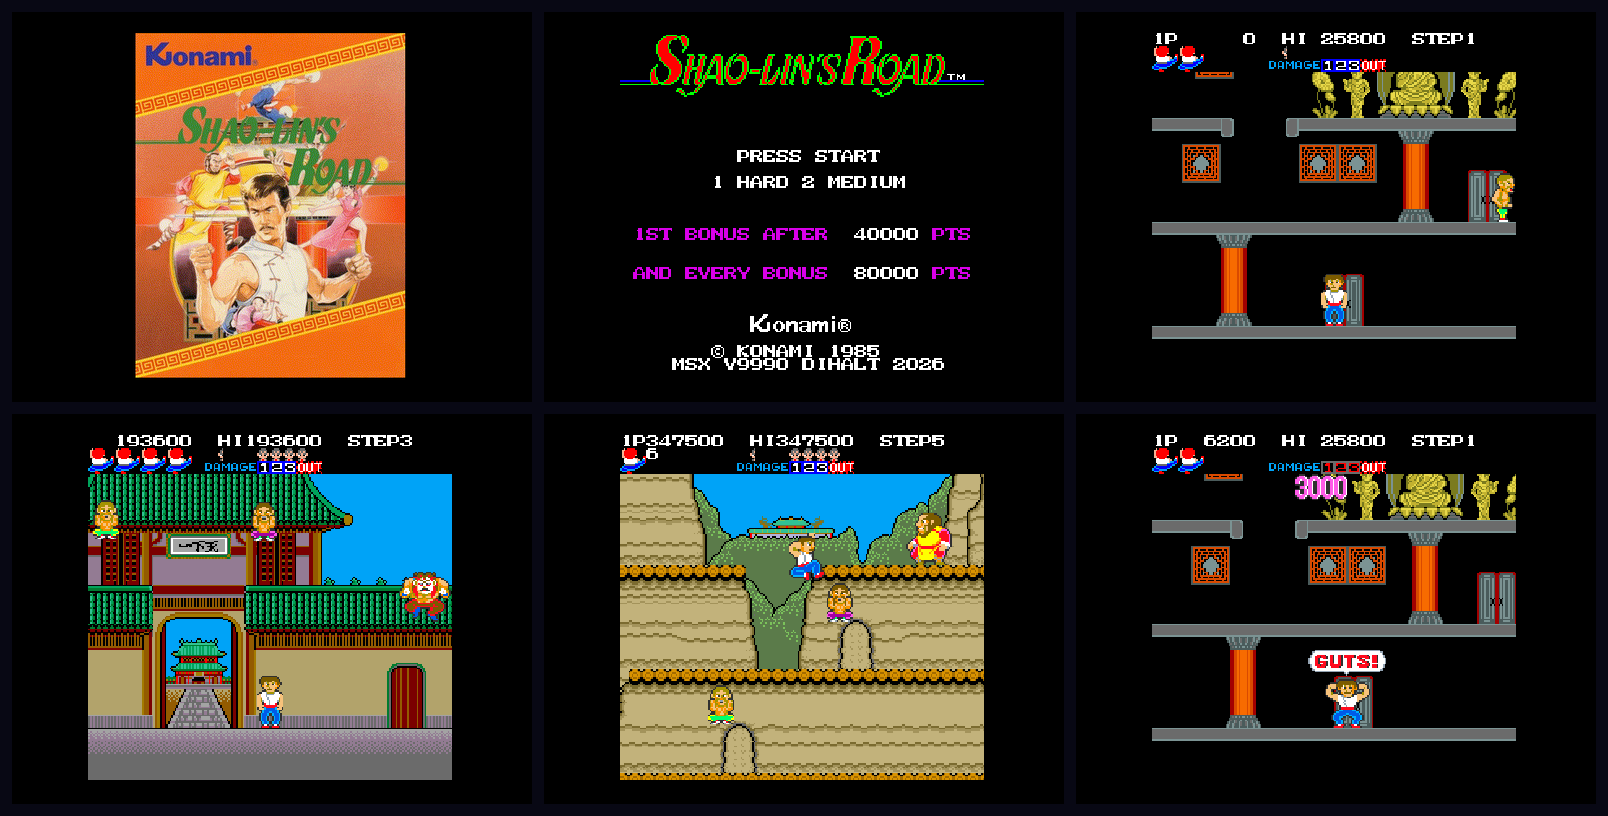
\includegraphics[width=0.8\textwidth]{img/montage.png}
\end{center}
\vfill
{\small \tHomage}
\newpage

\tableofcontents
\newpage

% ==================================================================
\sect{1. \tWhatYouNeed}

\begin{center}
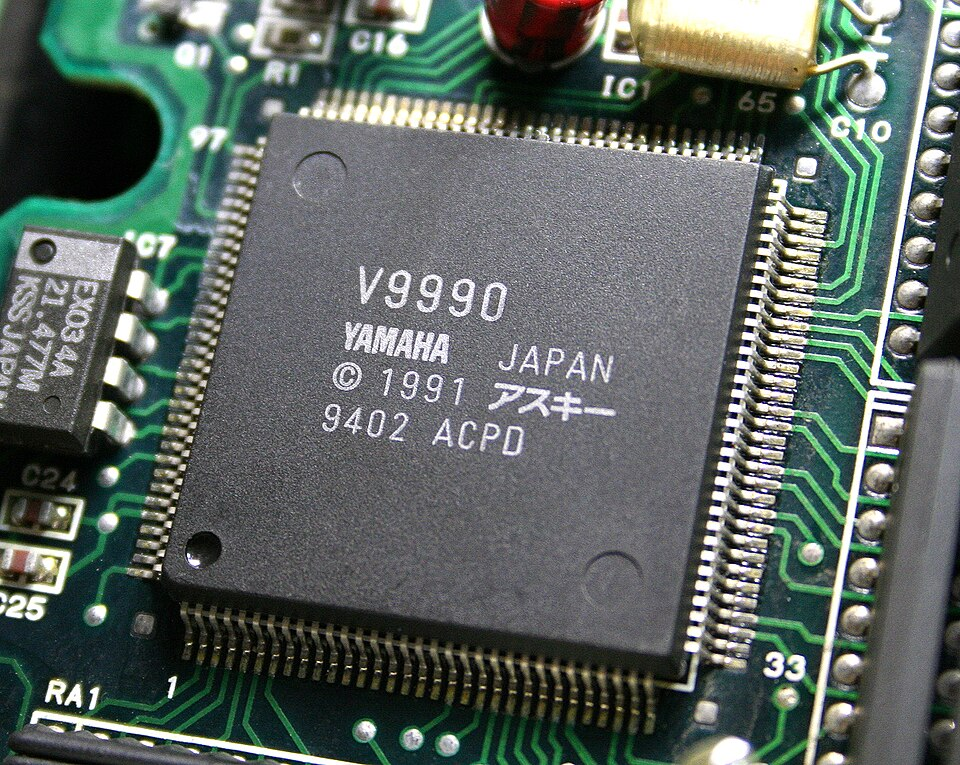
\includegraphics[width=0.62\textwidth]{img/v9990-chip.jpg}
\captionof{figure}{\tChipCaption{} Photo: Yaca2671, \href{https://commons.wikimedia.org/wiki/File:V9990_01.jpg}{Wikimedia Commons}, CC BY-SA 3.0.}
\end{center}

\begin{tabularx}{\textwidth}{@{}lX@{}}
\toprule
\textbf{\tItem} & \textbf{\tRequirement}\\
\midrule
\tComputer & \tComputerText\\
\tMemory & \tMemoryText\\
\tVideo & \tVideoText\\
\tSoundRow & \tSoundText\\
\tGameRow & \tGameText\\
\tMonitor & \tMonitorText\\
\tControlsRow & \tControlsText\\
\bottomrule
\end{tabularx}

\medskip
\tNoTape

% ==================================================================
\sect{2. \tSettingUp}

\begin{enumerate}
\item \tSetOff
\item \tSetV
\item \tSetGame
\item \tSetMonitor
\item \tSetJoy
\item \tSetOn
\end{enumerate}

\tBlackScreen

% ==================================================================
\sect{3. \tPowerOnTitle}

\begin{figure}[H]
\centering
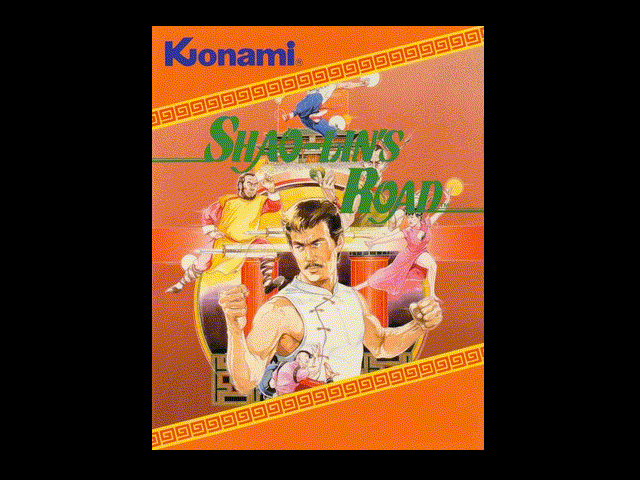
\includegraphics[width=0.48\textwidth]{img/cover-shot.png}\hfill
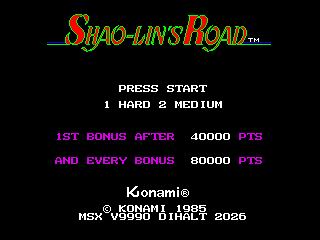
\includegraphics[width=0.48\textwidth]{img/title.png}
\caption{\tPowerOnCaption}
\end{figure}

\input{flow-\manlang}

% ==================================================================
\sect{4. \tControlsTitle}

\input{controls-\manlang}

% ==================================================================
\input{game-\manlang}

% ==================================================================
\sect{\tCreditsTitle}

\begin{itemize}
\item \textbf{\gameTitle} \tIsAGameBy{} \textbf{\originalPublisher}, \originalYear. \tRightsText
\item \textbf{\tVersionWord} (\portWork): \textbf{\portAuthor}, \portYear.
\item \tMsxTrademark{} (file \texttt{MSX-Logo.svg}, Wikimedia Commons).
\item \tChipNote
\item \tSourceNote
\end{itemize}

% ==================================================================
\newpage
\sect{\tAppendix}

\tStickerText

\begin{center}
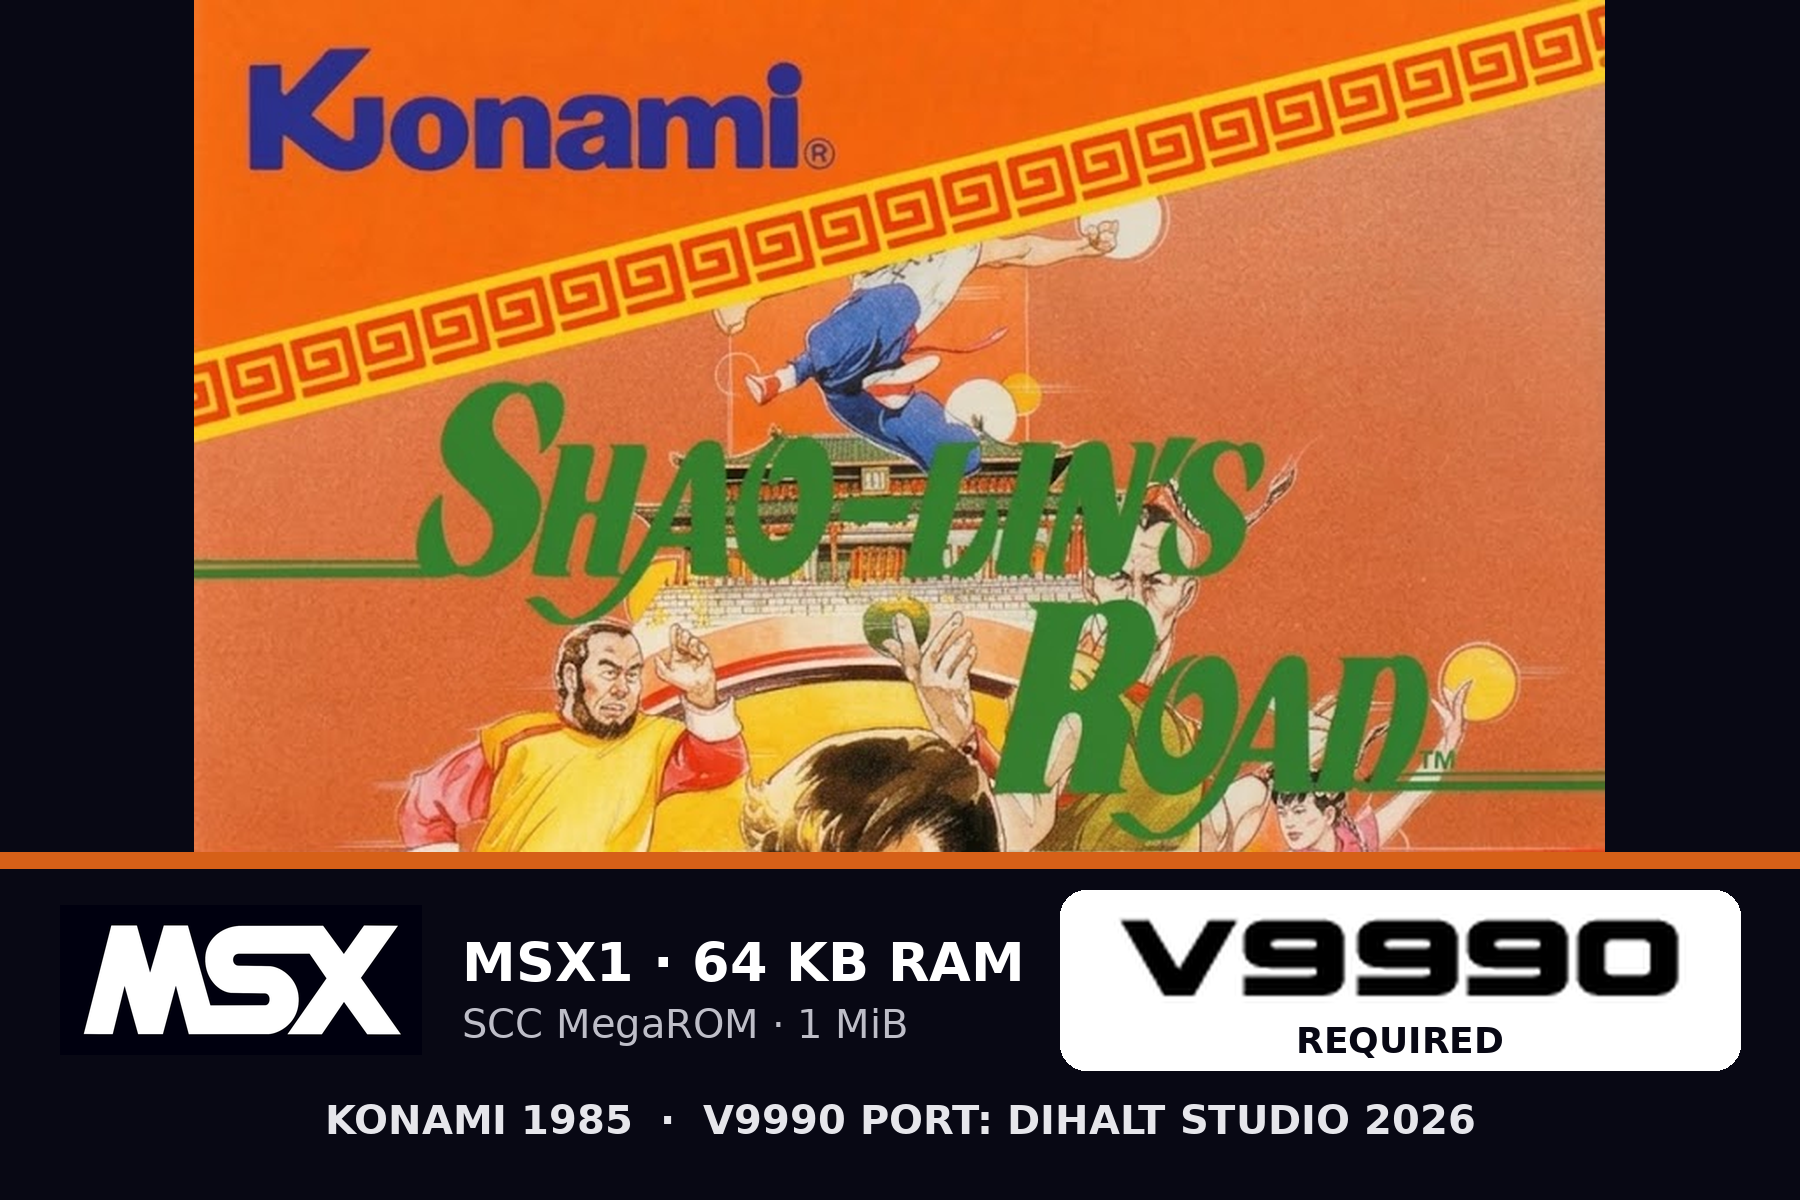
\includegraphics[width=\textwidth]{img/sticker.png}
\end{center}

\end{document}
"   (twice)
\documentclass[a4paper,11pt]{article}
\providecommand{\manlang}{en}
\usepackage[utf8]{inputenc}
\usepackage[T1]{fontenc}
\usepackage{lmodern,helvet}
\renewcommand{\familydefault}{\sfdefault}
% Facts about the game. Edit this file; manual.tex and the lang files read it.
\newcommand{\gameTitle}{Shao-lin's Road}
\newcommand{\originalPublisher}{Konami}
\newcommand{\originalYear}{1985}
\newcommand{\portAuthor}{DiHalt Studio}
\newcommand{\portYear}{2026}
\newcommand{\accentRGB}{214,96,24}      % accent colour of headings (R,G,B), taken from the cover
\newcommand{\romFile}{shaolins\_v9990.rom}
\newcommand{\romKind}{1~MiB Konami SCC MegaROM}   % mapper and size
\newcommand{\ramNeeded}{64~KB}
\newcommand{\portWork}{display engine, tools, title screen, cover conversion}  % what the port author did (EN)
\newcommand{\portWorkES}{motor de v\'ideo, herramientas, pantalla de t\'itulo, conversi\'on de la portada}

\InputIfFileExists{lang-\manlang}{}{\PackageError{manual}{no lang-\manlang.tex}{}}
\InputIfFileExists{override-\manlang}{}{}   % per-game replacements of the fixed texts
\usepackage[margin=2.2cm,top=2.4cm,bottom=2.4cm]{geometry}
\usepackage{graphicx,xcolor,booktabs,tabularx,float,caption,fancyhdr,eso-pic,parskip,microtype}
\usepackage[hidelinks,pdftitle={\gameTitle{} - \tManual},pdfauthor={\portAuthor}]{hyperref}

\definecolor{accent}{RGB}{\accentRGB}
\definecolor{ink}{RGB}{8,8,20}
\captionsetup{font=small,labelfont=bf}
\setlength{\parindent}{0pt}
\pagestyle{fancy}\fancyhf{}
\fancyhead[L]{\small\textcolor{accent}{\textbf{\MakeUppercase{\gameTitle}}} \tForV}
\fancyhead[R]{\small \tManual}
\fancyfoot[C]{\small\thepage}
\renewcommand{\headrulewidth}{0.4pt}

\newcommand{\key}[1]{{\fboxsep=2.5pt\fbox{\textbf{\strut #1}}}}
\newcommand{\sect}[1]{\section*{\textcolor{accent}{#1}}\addcontentsline{toc}{section}{#1}}

\begin{document}

% ---------- Cover: the game's cover picture, full page ----------
\thispagestyle{empty}
\AddToShipoutPictureBG*{\put(0,0){
\includegraphics[width=\paperwidth,height=\paperheight]{img/cover.jpg}}%
  \put(0.045\paperwidth,0.108\paperheight){
\includegraphics[width=0.30\paperwidth]{img/msx-logo.png}}%
  \put(0.045\paperwidth,0.05\paperheight){
\includegraphics[width=0.30\paperwidth]{img/v9990-logo.png}}}
\mbox{}\vfill
\begin{flushright}
\colorbox{ink}{\parbox{0.62\textwidth}{\raggedleft\color{white}\vspace{2pt}
{\Large\bfseries \tUserManual}\\[2pt]
{\large \tCoverLine}\vspace{4pt}}}
\end{flushright}
\newpage

% ---------- Title page ----------
\thispagestyle{empty}
\begin{center}
\vspace*{1.2cm}
{\fontsize{34}{38}\selectfont\bfseries\textcolor{accent}{\MakeUppercase{\gameTitle}}}\\[6pt]
{\Large \tForTheV}\\[1.0cm]

\includegraphics[height=2.2cm]{img/msx-logo.png}\hspace{1.2cm}
\includegraphics[height=1.5cm]{img/v9990-logo.png}\\[1.0cm]
\parbox{0.8\textwidth}{\centering
\tOriginalBy{} \textbf{\originalPublisher}, \originalYear.\\[3pt]
\tPortBy{} \textbf{\portAuthor}, \portYear.}\\[1.5cm]
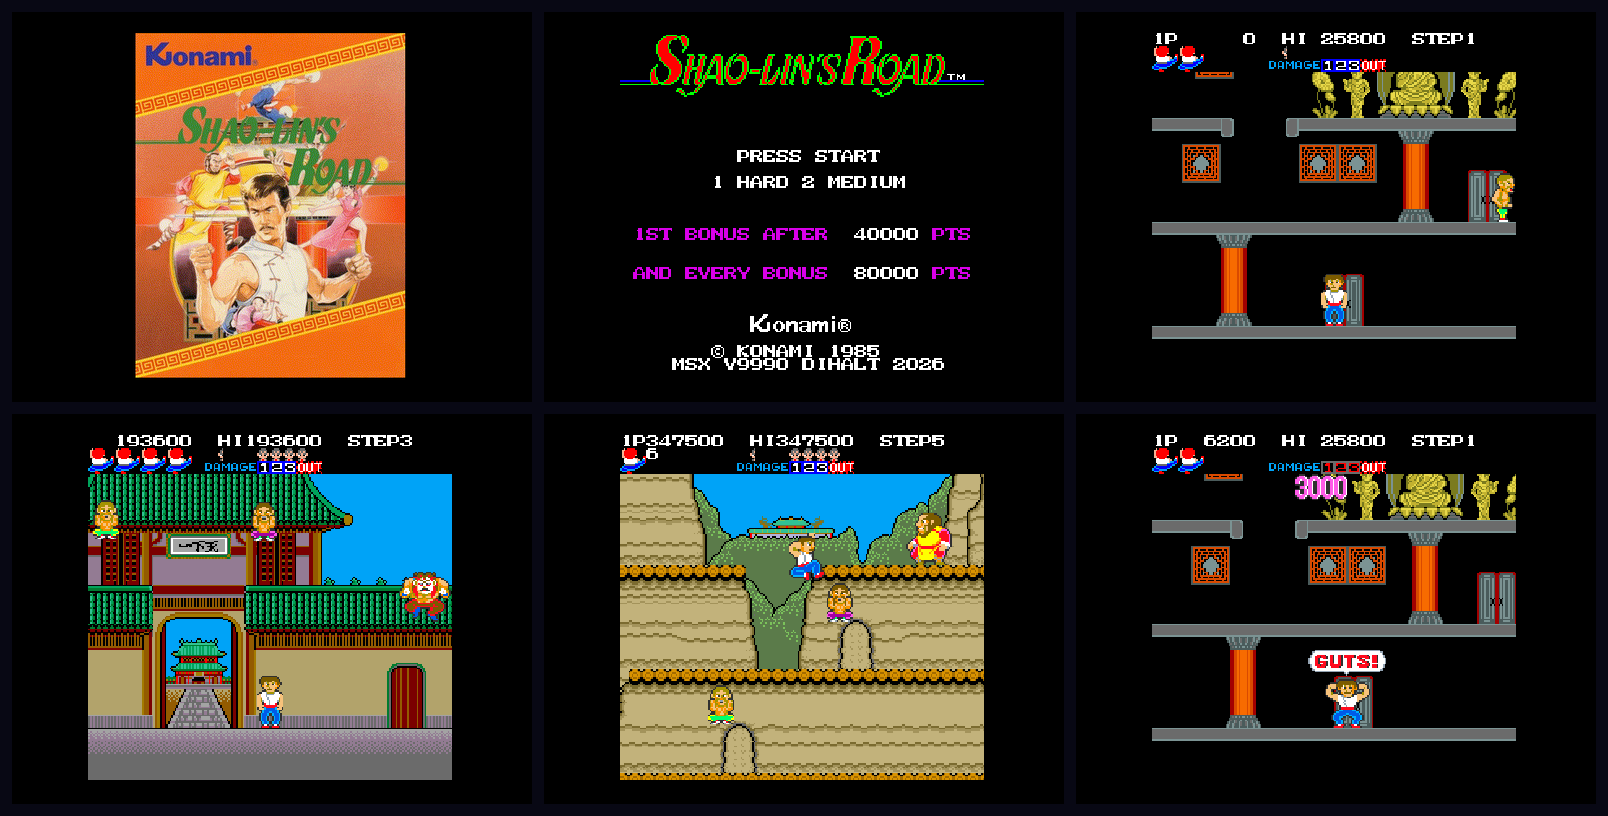
\includegraphics[width=0.8\textwidth]{img/montage.png}
\end{center}
\vfill
{\small \tHomage}
\newpage

\tableofcontents
\newpage

% ==================================================================
\sect{1. \tWhatYouNeed}

\begin{center}
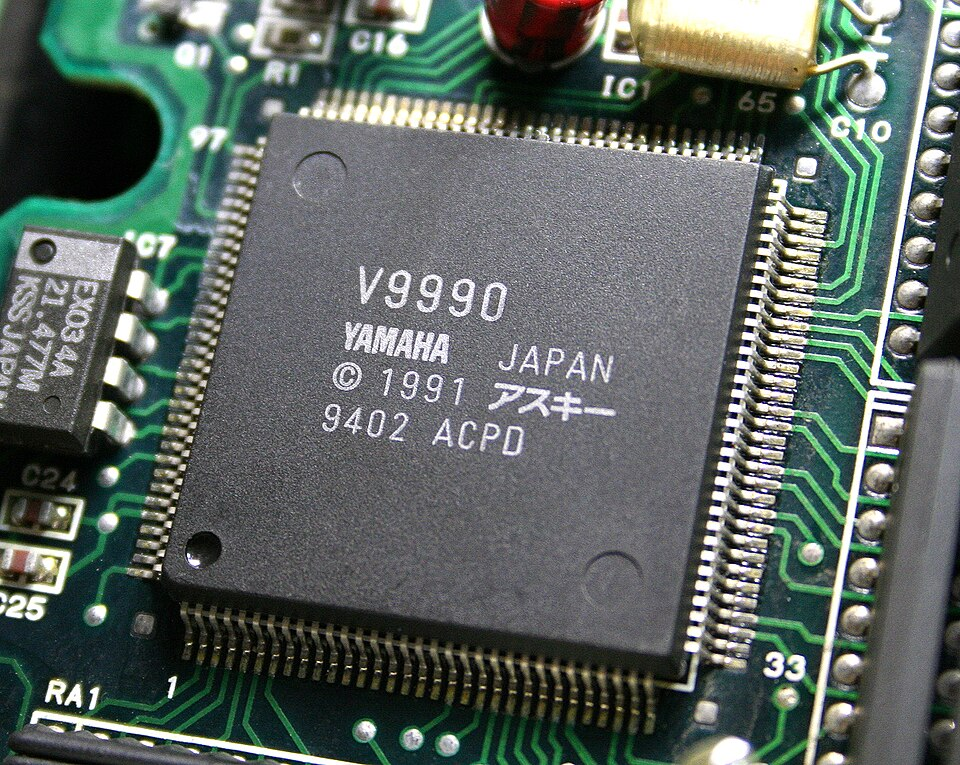
\includegraphics[width=0.62\textwidth]{img/v9990-chip.jpg}
\captionof{figure}{\tChipCaption{} Photo: Yaca2671, \href{https://commons.wikimedia.org/wiki/File:V9990_01.jpg}{Wikimedia Commons}, CC BY-SA 3.0.}
\end{center}

\begin{tabularx}{\textwidth}{@{}lX@{}}
\toprule
\textbf{\tItem} & \textbf{\tRequirement}\\
\midrule
\tComputer & \tComputerText\\
\tMemory & \tMemoryText\\
\tVideo & \tVideoText\\
\tSoundRow & \tSoundText\\
\tGameRow & \tGameText\\
\tMonitor & \tMonitorText\\
\tControlsRow & \tControlsText\\
\bottomrule
\end{tabularx}

\medskip
\tNoTape

% ==================================================================
\sect{2. \tSettingUp}

\begin{enumerate}
\item \tSetOff
\item \tSetV
\item \tSetGame
\item \tSetMonitor
\item \tSetJoy
\item \tSetOn
\end{enumerate}

\tBlackScreen

% ==================================================================
\sect{3. \tPowerOnTitle}

\begin{figure}[H]
\centering
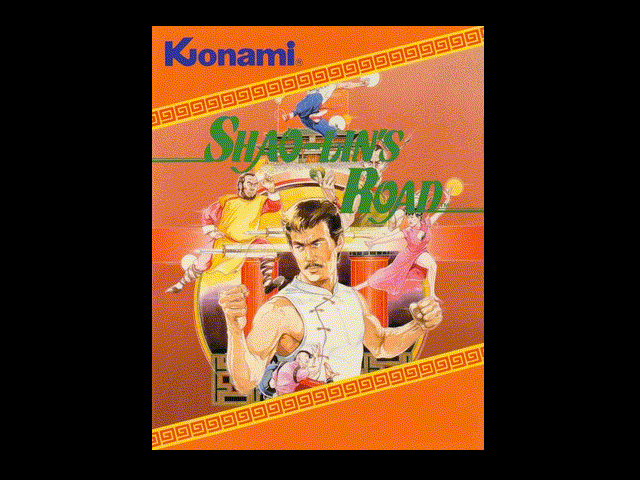
\includegraphics[width=0.48\textwidth]{img/cover-shot.png}\hfill
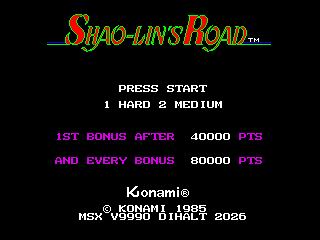
\includegraphics[width=0.48\textwidth]{img/title.png}
\caption{\tPowerOnCaption}
\end{figure}

\input{flow-\manlang}

% ==================================================================
\sect{4. \tControlsTitle}

\input{controls-\manlang}

% ==================================================================
\input{game-\manlang}

% ==================================================================
\sect{\tCreditsTitle}

\begin{itemize}
\item \textbf{\gameTitle} \tIsAGameBy{} \textbf{\originalPublisher}, \originalYear. \tRightsText
\item \textbf{\tVersionWord} (\portWork): \textbf{\portAuthor}, \portYear.
\item \tMsxTrademark{} (file \texttt{MSX-Logo.svg}, Wikimedia Commons).
\item \tChipNote
\item \tSourceNote
\end{itemize}

% ==================================================================
\newpage
\sect{\tAppendix}

\tStickerText

\begin{center}
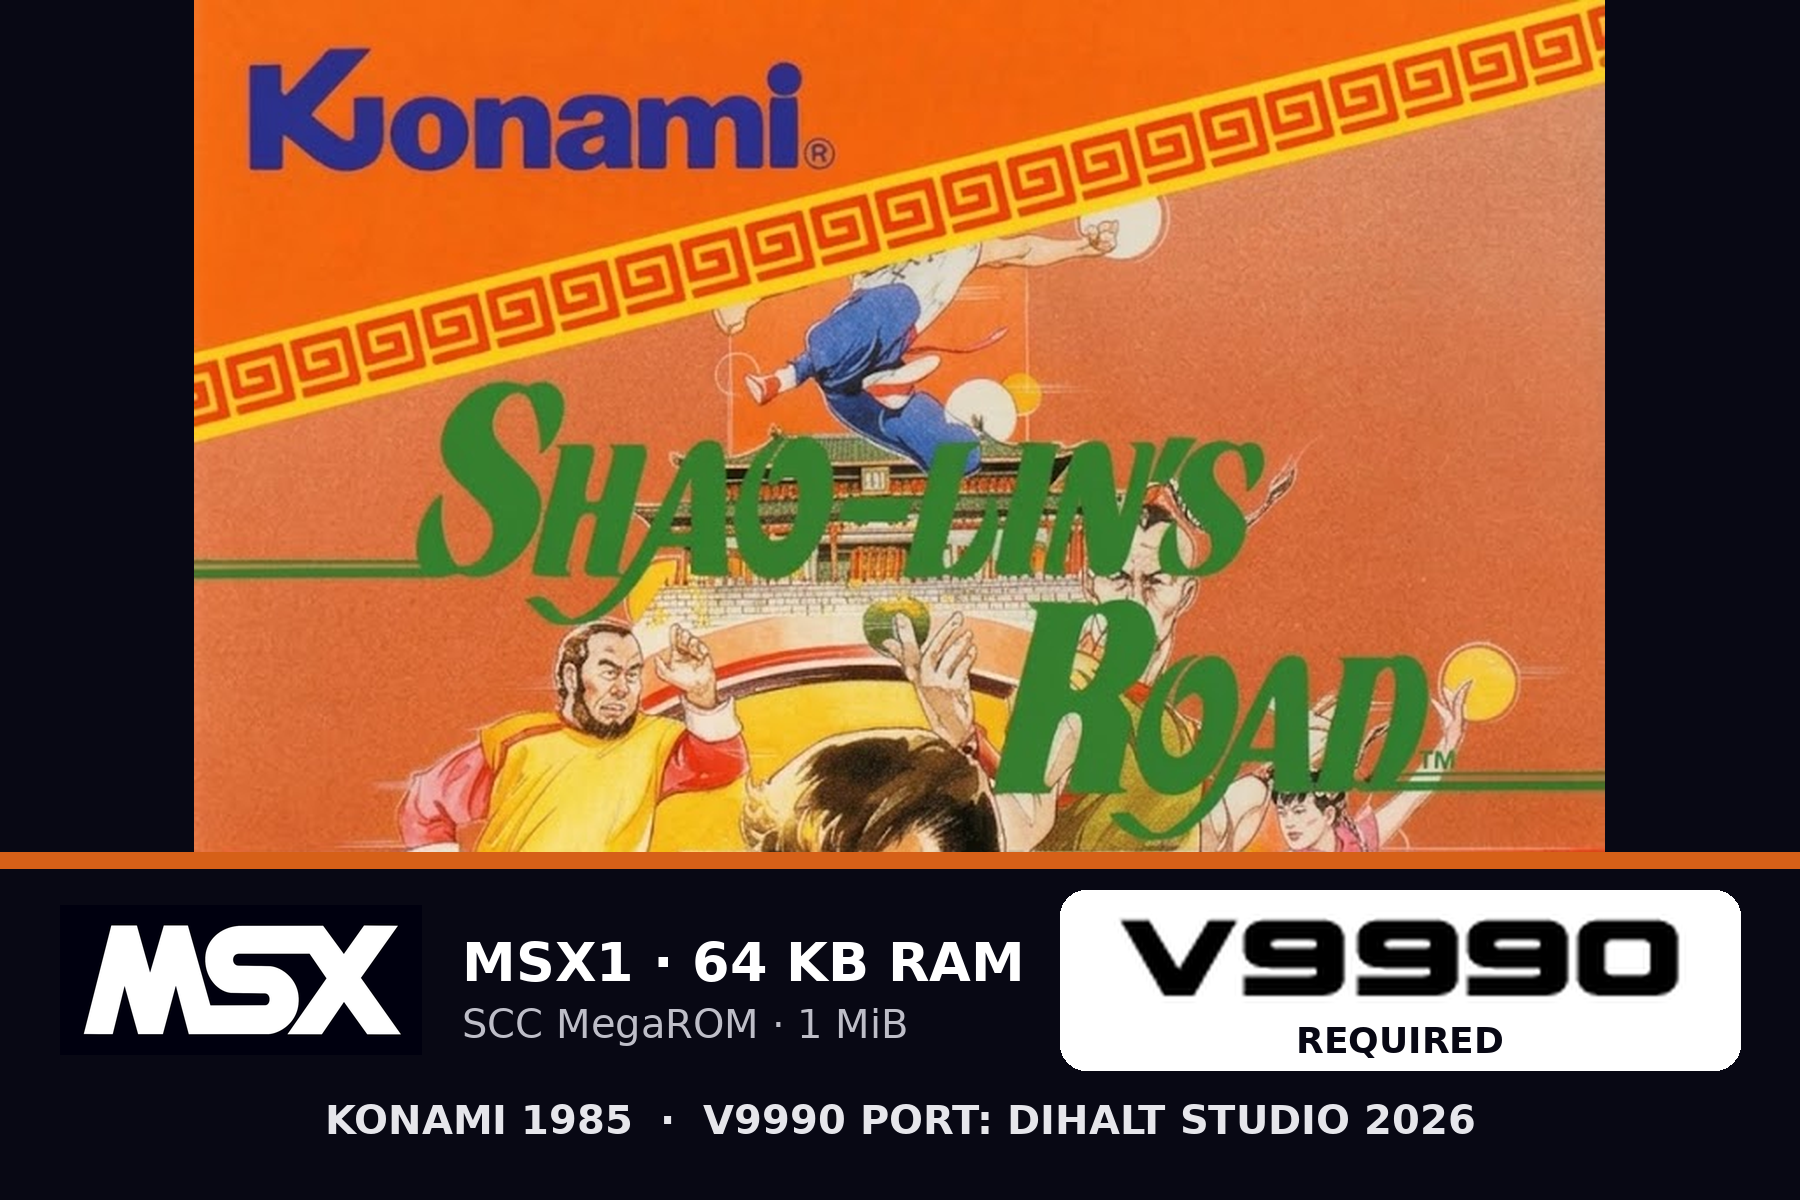
\includegraphics[width=\textwidth]{img/sticker.png}
\end{center}

\end{document}
"   (twice)
\documentclass[a4paper,11pt]{article}
\providecommand{\manlang}{en}
\usepackage[utf8]{inputenc}
\usepackage[T1]{fontenc}
\usepackage{lmodern,helvet}
\renewcommand{\familydefault}{\sfdefault}
% Facts about the game. Edit this file; manual.tex and the lang files read it.
\newcommand{\gameTitle}{Shao-lin's Road}
\newcommand{\originalPublisher}{Konami}
\newcommand{\originalYear}{1985}
\newcommand{\portAuthor}{DiHalt Studio}
\newcommand{\portYear}{2026}
\newcommand{\accentRGB}{214,96,24}      % accent colour of headings (R,G,B), taken from the cover
\newcommand{\romFile}{shaolins\_v9990.rom}
\newcommand{\romKind}{1~MiB Konami SCC MegaROM}   % mapper and size
\newcommand{\ramNeeded}{64~KB}
\newcommand{\portWork}{display engine, tools, title screen, cover conversion}  % what the port author did (EN)
\newcommand{\portWorkES}{motor de v\'ideo, herramientas, pantalla de t\'itulo, conversi\'on de la portada}

\InputIfFileExists{lang-\manlang}{}{\PackageError{manual}{no lang-\manlang.tex}{}}
\InputIfFileExists{override-\manlang}{}{}   % per-game replacements of the fixed texts
\usepackage[margin=2.2cm,top=2.4cm,bottom=2.4cm]{geometry}
\usepackage{graphicx,xcolor,booktabs,tabularx,float,caption,fancyhdr,eso-pic,parskip,microtype}
\usepackage[hidelinks,pdftitle={\gameTitle{} - \tManual},pdfauthor={\portAuthor}]{hyperref}

\definecolor{accent}{RGB}{\accentRGB}
\definecolor{ink}{RGB}{8,8,20}
\captionsetup{font=small,labelfont=bf}
\setlength{\parindent}{0pt}
\pagestyle{fancy}\fancyhf{}
\fancyhead[L]{\small\textcolor{accent}{\textbf{\MakeUppercase{\gameTitle}}} \tForV}
\fancyhead[R]{\small \tManual}
\fancyfoot[C]{\small\thepage}
\renewcommand{\headrulewidth}{0.4pt}

\newcommand{\key}[1]{{\fboxsep=2.5pt\fbox{\textbf{\strut #1}}}}
\newcommand{\sect}[1]{\section*{\textcolor{accent}{#1}}\addcontentsline{toc}{section}{#1}}

\begin{document}

% ---------- Cover: the game's cover picture, full page ----------
\thispagestyle{empty}
\AddToShipoutPictureBG*{\put(0,0){
\includegraphics[width=\paperwidth,height=\paperheight]{img/cover.jpg}}%
  \put(0.045\paperwidth,0.108\paperheight){
\includegraphics[width=0.30\paperwidth]{img/msx-logo.png}}%
  \put(0.045\paperwidth,0.05\paperheight){
\includegraphics[width=0.30\paperwidth]{img/v9990-logo.png}}}
\mbox{}\vfill
\begin{flushright}
\colorbox{ink}{\parbox{0.62\textwidth}{\raggedleft\color{white}\vspace{2pt}
{\Large\bfseries \tUserManual}\\[2pt]
{\large \tCoverLine}\vspace{4pt}}}
\end{flushright}
\newpage

% ---------- Title page ----------
\thispagestyle{empty}
\begin{center}
\vspace*{1.2cm}
{\fontsize{34}{38}\selectfont\bfseries\textcolor{accent}{\MakeUppercase{\gameTitle}}}\\[6pt]
{\Large \tForTheV}\\[1.0cm]

\includegraphics[height=2.2cm]{img/msx-logo.png}\hspace{1.2cm}
\includegraphics[height=1.5cm]{img/v9990-logo.png}\\[1.0cm]
\parbox{0.8\textwidth}{\centering
\tOriginalBy{} \textbf{\originalPublisher}, \originalYear.\\[3pt]
\tPortBy{} \textbf{\portAuthor}, \portYear.}\\[1.5cm]
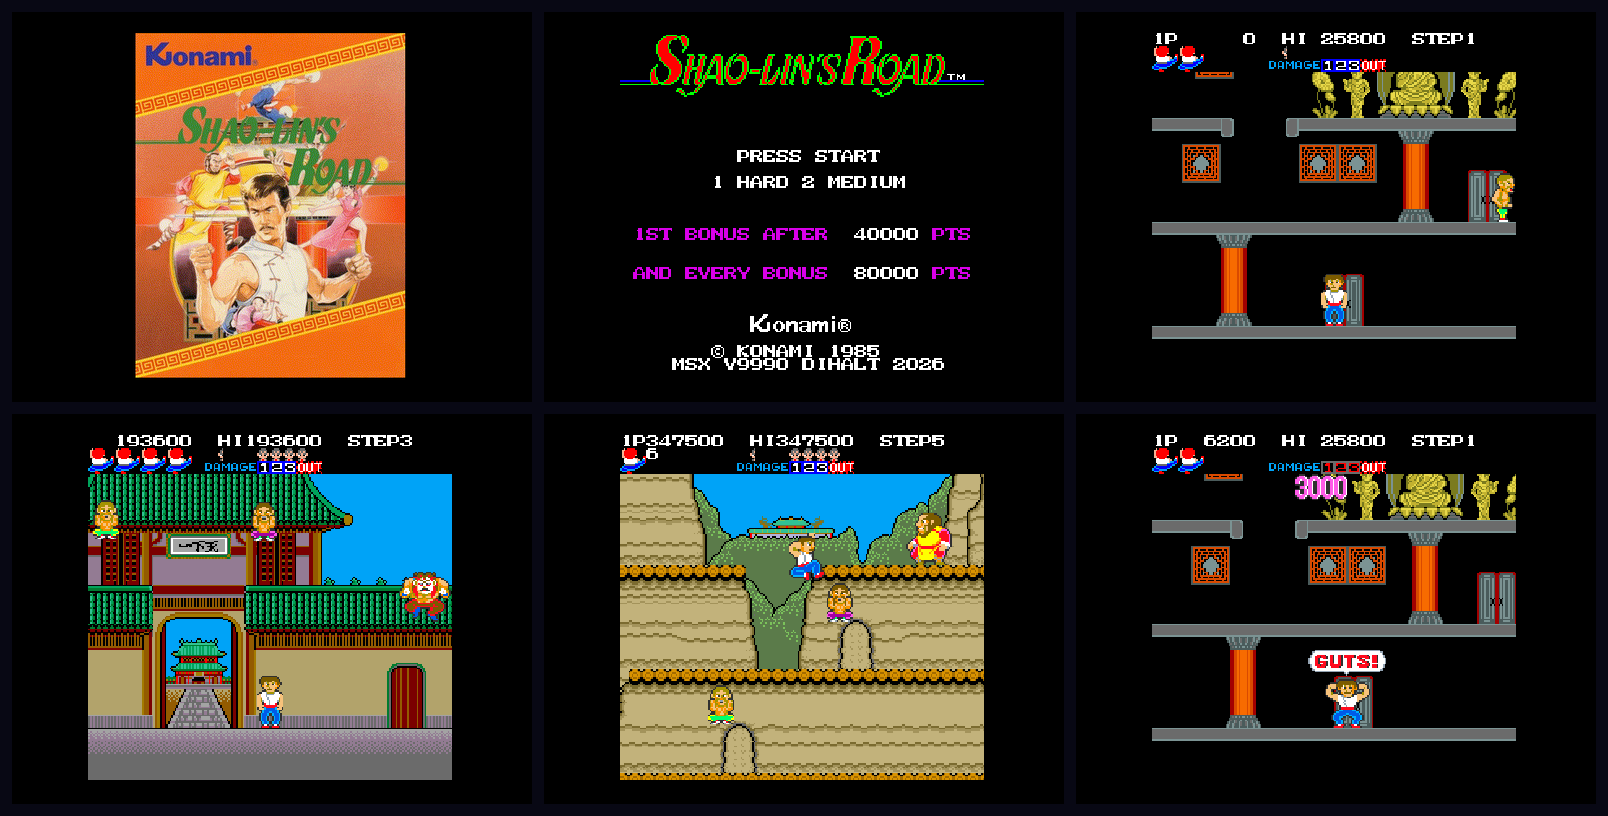
\includegraphics[width=0.8\textwidth]{img/montage.png}
\end{center}
\vfill
{\small \tHomage}
\newpage

\tableofcontents
\newpage

% ==================================================================
\sect{1. \tWhatYouNeed}

\begin{center}
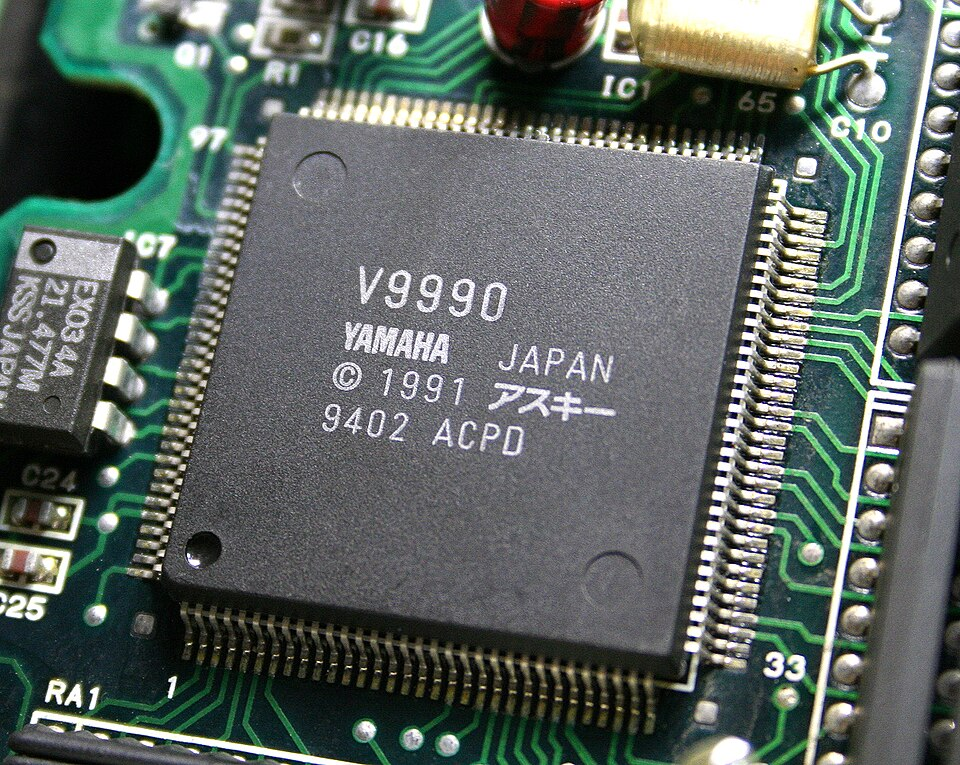
\includegraphics[width=0.62\textwidth]{img/v9990-chip.jpg}
\captionof{figure}{\tChipCaption{} Photo: Yaca2671, \href{https://commons.wikimedia.org/wiki/File:V9990_01.jpg}{Wikimedia Commons}, CC BY-SA 3.0.}
\end{center}

\begin{tabularx}{\textwidth}{@{}lX@{}}
\toprule
\textbf{\tItem} & \textbf{\tRequirement}\\
\midrule
\tComputer & \tComputerText\\
\tMemory & \tMemoryText\\
\tVideo & \tVideoText\\
\tSoundRow & \tSoundText\\
\tGameRow & \tGameText\\
\tMonitor & \tMonitorText\\
\tControlsRow & \tControlsText\\
\bottomrule
\end{tabularx}

\medskip
\tNoTape

% ==================================================================
\sect{2. \tSettingUp}

\begin{enumerate}
\item \tSetOff
\item \tSetV
\item \tSetGame
\item \tSetMonitor
\item \tSetJoy
\item \tSetOn
\end{enumerate}

\tBlackScreen

% ==================================================================
\sect{3. \tPowerOnTitle}

\begin{figure}[H]
\centering
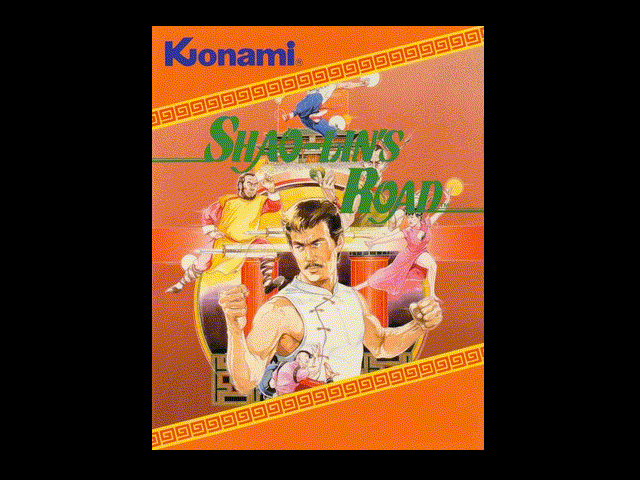
\includegraphics[width=0.48\textwidth]{img/cover-shot.png}\hfill
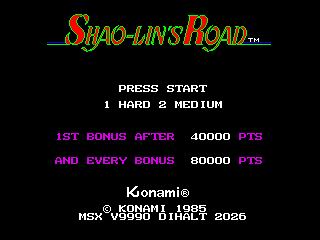
\includegraphics[width=0.48\textwidth]{img/title.png}
\caption{\tPowerOnCaption}
\end{figure}

\input{flow-\manlang}

% ==================================================================
\sect{4. \tControlsTitle}

\input{controls-\manlang}

% ==================================================================
\input{game-\manlang}

% ==================================================================
\sect{\tCreditsTitle}

\begin{itemize}
\item \textbf{\gameTitle} \tIsAGameBy{} \textbf{\originalPublisher}, \originalYear. \tRightsText
\item \textbf{\tVersionWord} (\portWork): \textbf{\portAuthor}, \portYear.
\item \tMsxTrademark{} (file \texttt{MSX-Logo.svg}, Wikimedia Commons).
\item \tChipNote
\item \tSourceNote
\end{itemize}

% ==================================================================
\newpage
\sect{\tAppendix}

\tStickerText

\begin{center}
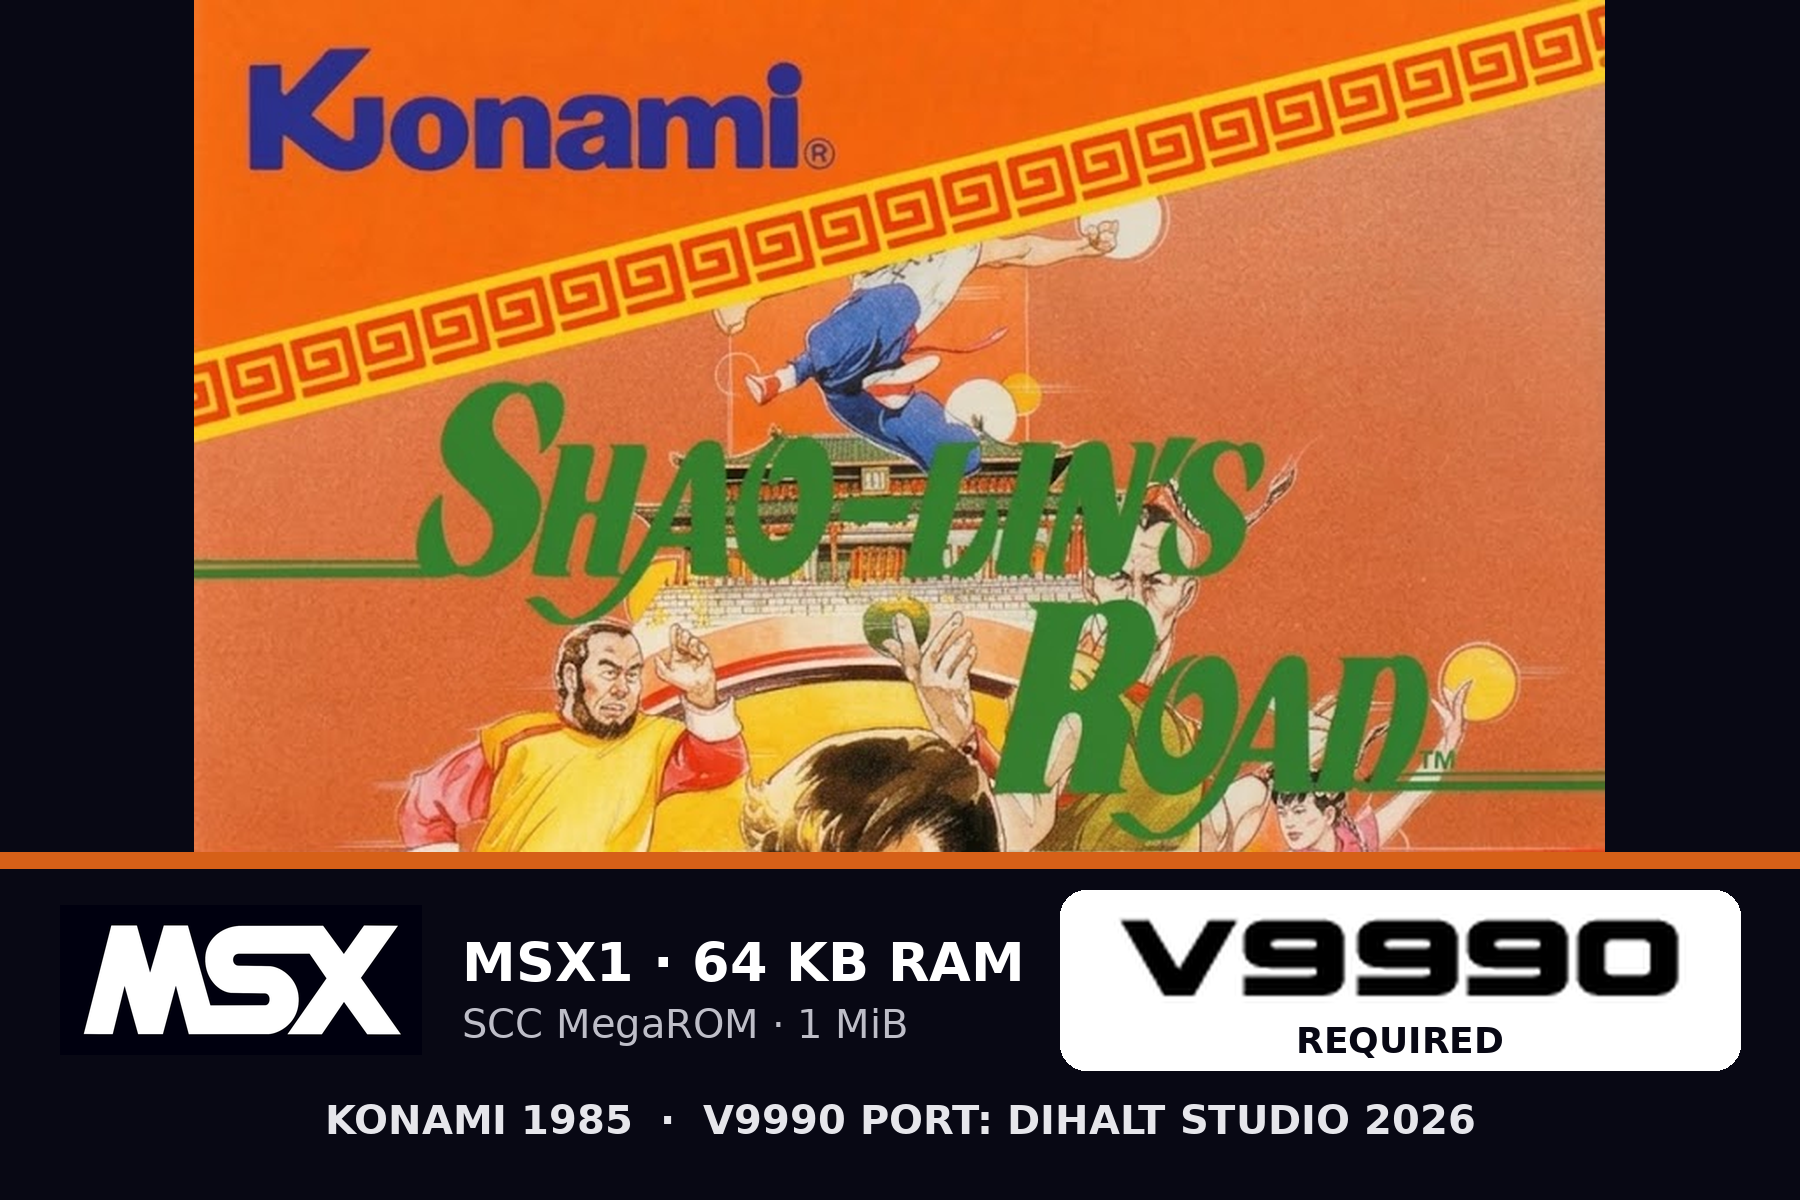
\includegraphics[width=\textwidth]{img/sticker.png}
\end{center}

\end{document}
"   (twice)
\documentclass[a4paper,11pt]{article}
\providecommand{\manlang}{en}
\usepackage[utf8]{inputenc}
\usepackage[T1]{fontenc}
\usepackage{lmodern,helvet}
\renewcommand{\familydefault}{\sfdefault}
% Facts about the game. Edit this file; manual.tex and the lang files read it.
\newcommand{\gameTitle}{Shao-lin's Road}
\newcommand{\originalPublisher}{Konami}
\newcommand{\originalYear}{1985}
\newcommand{\portAuthor}{DiHalt Studio}
\newcommand{\portYear}{2026}
\newcommand{\accentRGB}{214,96,24}      % accent colour of headings (R,G,B), taken from the cover
\newcommand{\romFile}{shaolins\_v9990.rom}
\newcommand{\romKind}{1~MiB Konami SCC MegaROM}   % mapper and size
\newcommand{\ramNeeded}{64~KB}
\newcommand{\portWork}{display engine, tools, title screen, cover conversion}  % what the port author did (EN)
\newcommand{\portWorkES}{motor de v\'ideo, herramientas, pantalla de t\'itulo, conversi\'on de la portada}

\InputIfFileExists{lang-\manlang}{}{\PackageError{manual}{no lang-\manlang.tex}{}}
\InputIfFileExists{override-\manlang}{}{}   % per-game replacements of the fixed texts
\usepackage[margin=2.2cm,top=2.4cm,bottom=2.4cm]{geometry}
\usepackage{graphicx,xcolor,booktabs,tabularx,float,caption,fancyhdr,eso-pic,parskip,microtype}
\usepackage[hidelinks,pdftitle={\gameTitle{} - \tManual},pdfauthor={\portAuthor}]{hyperref}

\definecolor{accent}{RGB}{\accentRGB}
\definecolor{ink}{RGB}{8,8,20}
\captionsetup{font=small,labelfont=bf}
\setlength{\parindent}{0pt}
\pagestyle{fancy}\fancyhf{}
\fancyhead[L]{\small\textcolor{accent}{\textbf{\MakeUppercase{\gameTitle}}} \tForV}
\fancyhead[R]{\small \tManual}
\fancyfoot[C]{\small\thepage}
\renewcommand{\headrulewidth}{0.4pt}

\newcommand{\key}[1]{{\fboxsep=2.5pt\fbox{\textbf{\strut #1}}}}
\newcommand{\sect}[1]{\section*{\textcolor{accent}{#1}}\addcontentsline{toc}{section}{#1}}

\begin{document}

% ---------- Cover: the game's cover picture, full page ----------
\thispagestyle{empty}
\AddToShipoutPictureBG*{\put(0,0){
\includegraphics[width=\paperwidth,height=\paperheight]{img/cover.jpg}}%
  \put(0.045\paperwidth,0.108\paperheight){
\includegraphics[width=0.30\paperwidth]{img/msx-logo.png}}%
  \put(0.045\paperwidth,0.05\paperheight){
\includegraphics[width=0.30\paperwidth]{img/v9990-logo.png}}}
\mbox{}\vfill
\begin{flushright}
\colorbox{ink}{\parbox{0.62\textwidth}{\raggedleft\color{white}\vspace{2pt}
{\Large\bfseries \tUserManual}\\[2pt]
{\large \tCoverLine}\vspace{4pt}}}
\end{flushright}
\newpage

% ---------- Title page ----------
\thispagestyle{empty}
\begin{center}
\vspace*{1.2cm}
{\fontsize{34}{38}\selectfont\bfseries\textcolor{accent}{\MakeUppercase{\gameTitle}}}\\[6pt]
{\Large \tForTheV}\\[1.0cm]

\includegraphics[height=2.2cm]{img/msx-logo.png}\hspace{1.2cm}
\includegraphics[height=1.5cm]{img/v9990-logo.png}\\[1.0cm]
\parbox{0.8\textwidth}{\centering
\tOriginalBy{} \textbf{\originalPublisher}, \originalYear.\\[3pt]
\tPortBy{} \textbf{\portAuthor}, \portYear.}\\[1.5cm]
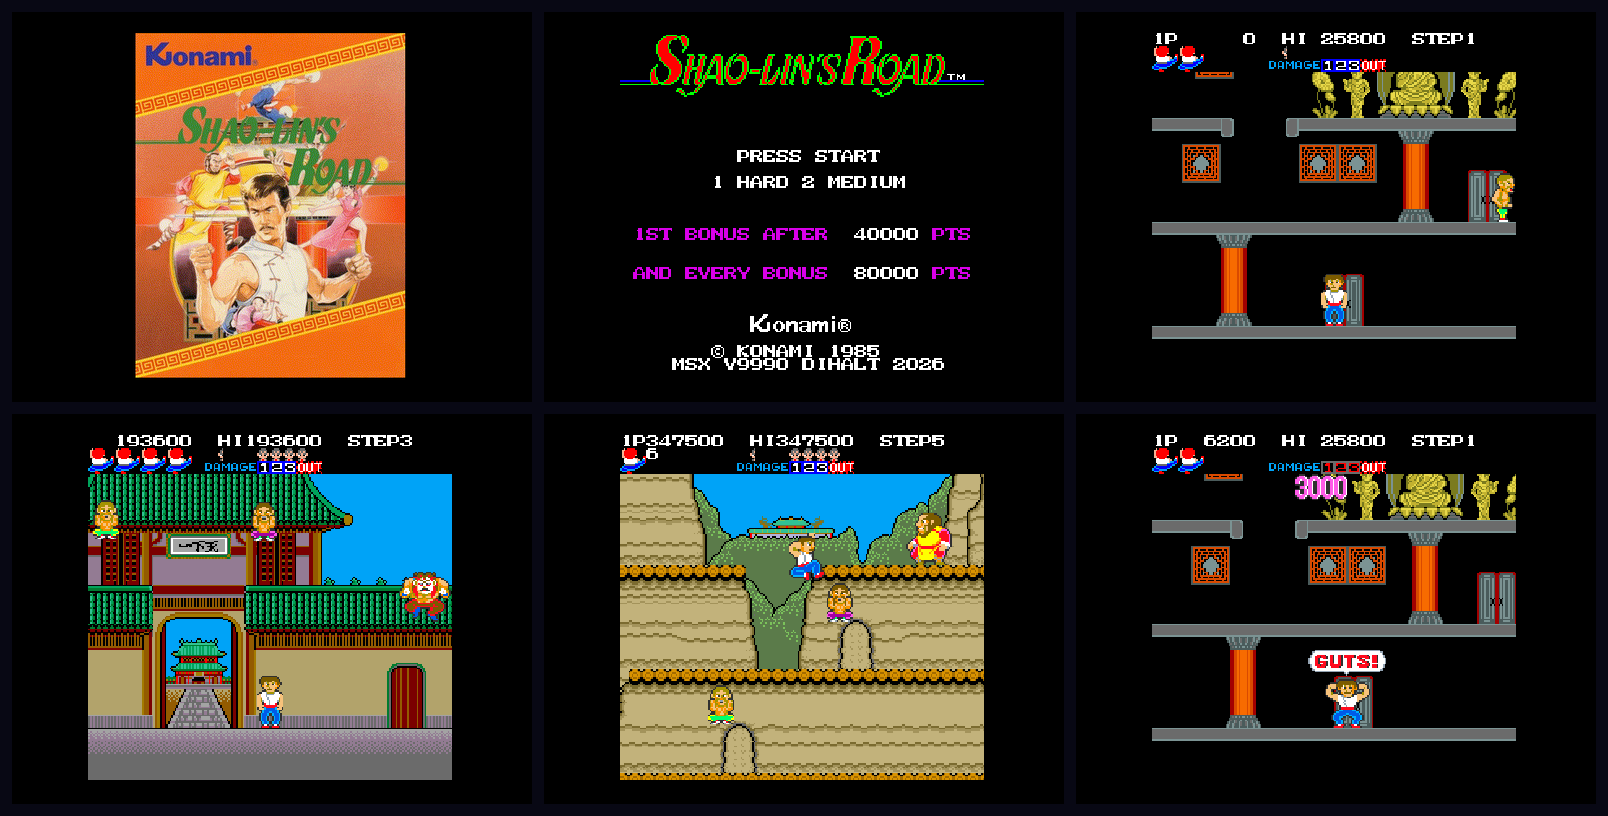
\includegraphics[width=0.8\textwidth]{img/montage.png}
\end{center}
\vfill
{\small \tHomage}
\newpage

\tableofcontents
\newpage

% ==================================================================
\sect{1. \tWhatYouNeed}

\begin{center}
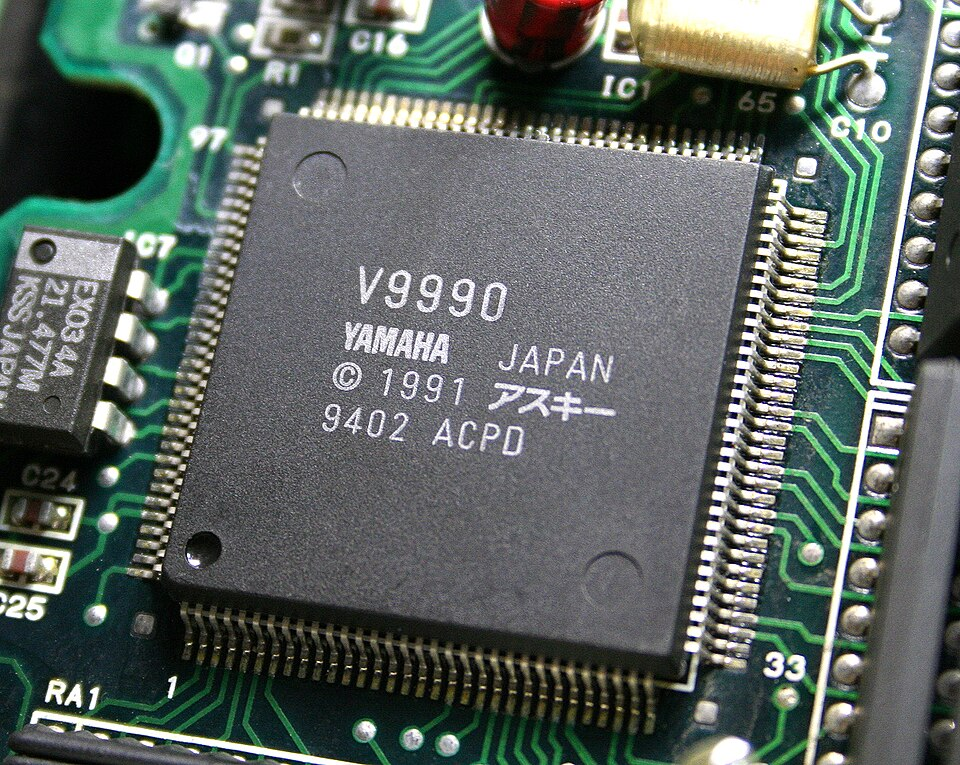
\includegraphics[width=0.62\textwidth]{img/v9990-chip.jpg}
\captionof{figure}{\tChipCaption{} Photo: Yaca2671, \href{https://commons.wikimedia.org/wiki/File:V9990_01.jpg}{Wikimedia Commons}, CC BY-SA 3.0.}
\end{center}

\begin{tabularx}{\textwidth}{@{}lX@{}}
\toprule
\textbf{\tItem} & \textbf{\tRequirement}\\
\midrule
\tComputer & \tComputerText\\
\tMemory & \tMemoryText\\
\tVideo & \tVideoText\\
\tSoundRow & \tSoundText\\
\tGameRow & \tGameText\\
\tMonitor & \tMonitorText\\
\tControlsRow & \tControlsText\\
\bottomrule
\end{tabularx}

\medskip
\tNoTape

% ==================================================================
\sect{2. \tSettingUp}

\begin{enumerate}
\item \tSetOff
\item \tSetV
\item \tSetGame
\item \tSetMonitor
\item \tSetJoy
\item \tSetOn
\end{enumerate}

\tBlackScreen

% ==================================================================
\sect{3. \tPowerOnTitle}

\begin{figure}[H]
\centering
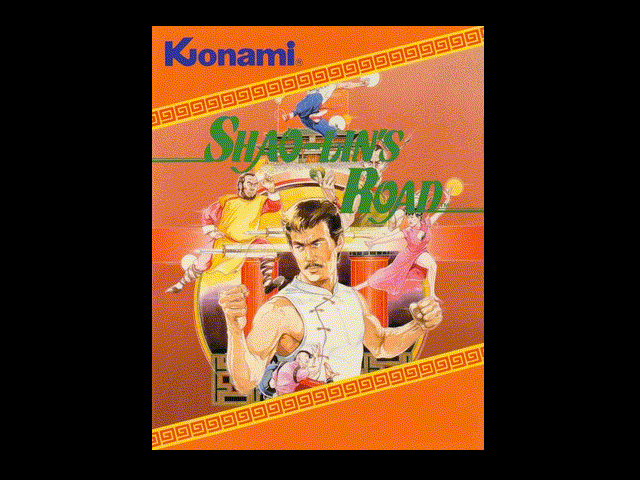
\includegraphics[width=0.48\textwidth]{img/cover-shot.png}\hfill
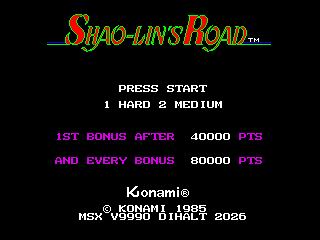
\includegraphics[width=0.48\textwidth]{img/title.png}
\caption{\tPowerOnCaption}
\end{figure}

\input{flow-\manlang}

% ==================================================================
\sect{4. \tControlsTitle}

\input{controls-\manlang}

% ==================================================================
\input{game-\manlang}

% ==================================================================
\sect{\tCreditsTitle}

\begin{itemize}
\item \textbf{\gameTitle} \tIsAGameBy{} \textbf{\originalPublisher}, \originalYear. \tRightsText
\item \textbf{\tVersionWord} (\portWork): \textbf{\portAuthor}, \portYear.
\item \tMsxTrademark{} (file \texttt{MSX-Logo.svg}, Wikimedia Commons).
\item \tChipNote
\item \tSourceNote
\end{itemize}

% ==================================================================
\newpage
\sect{\tAppendix}

\tStickerText

\begin{center}
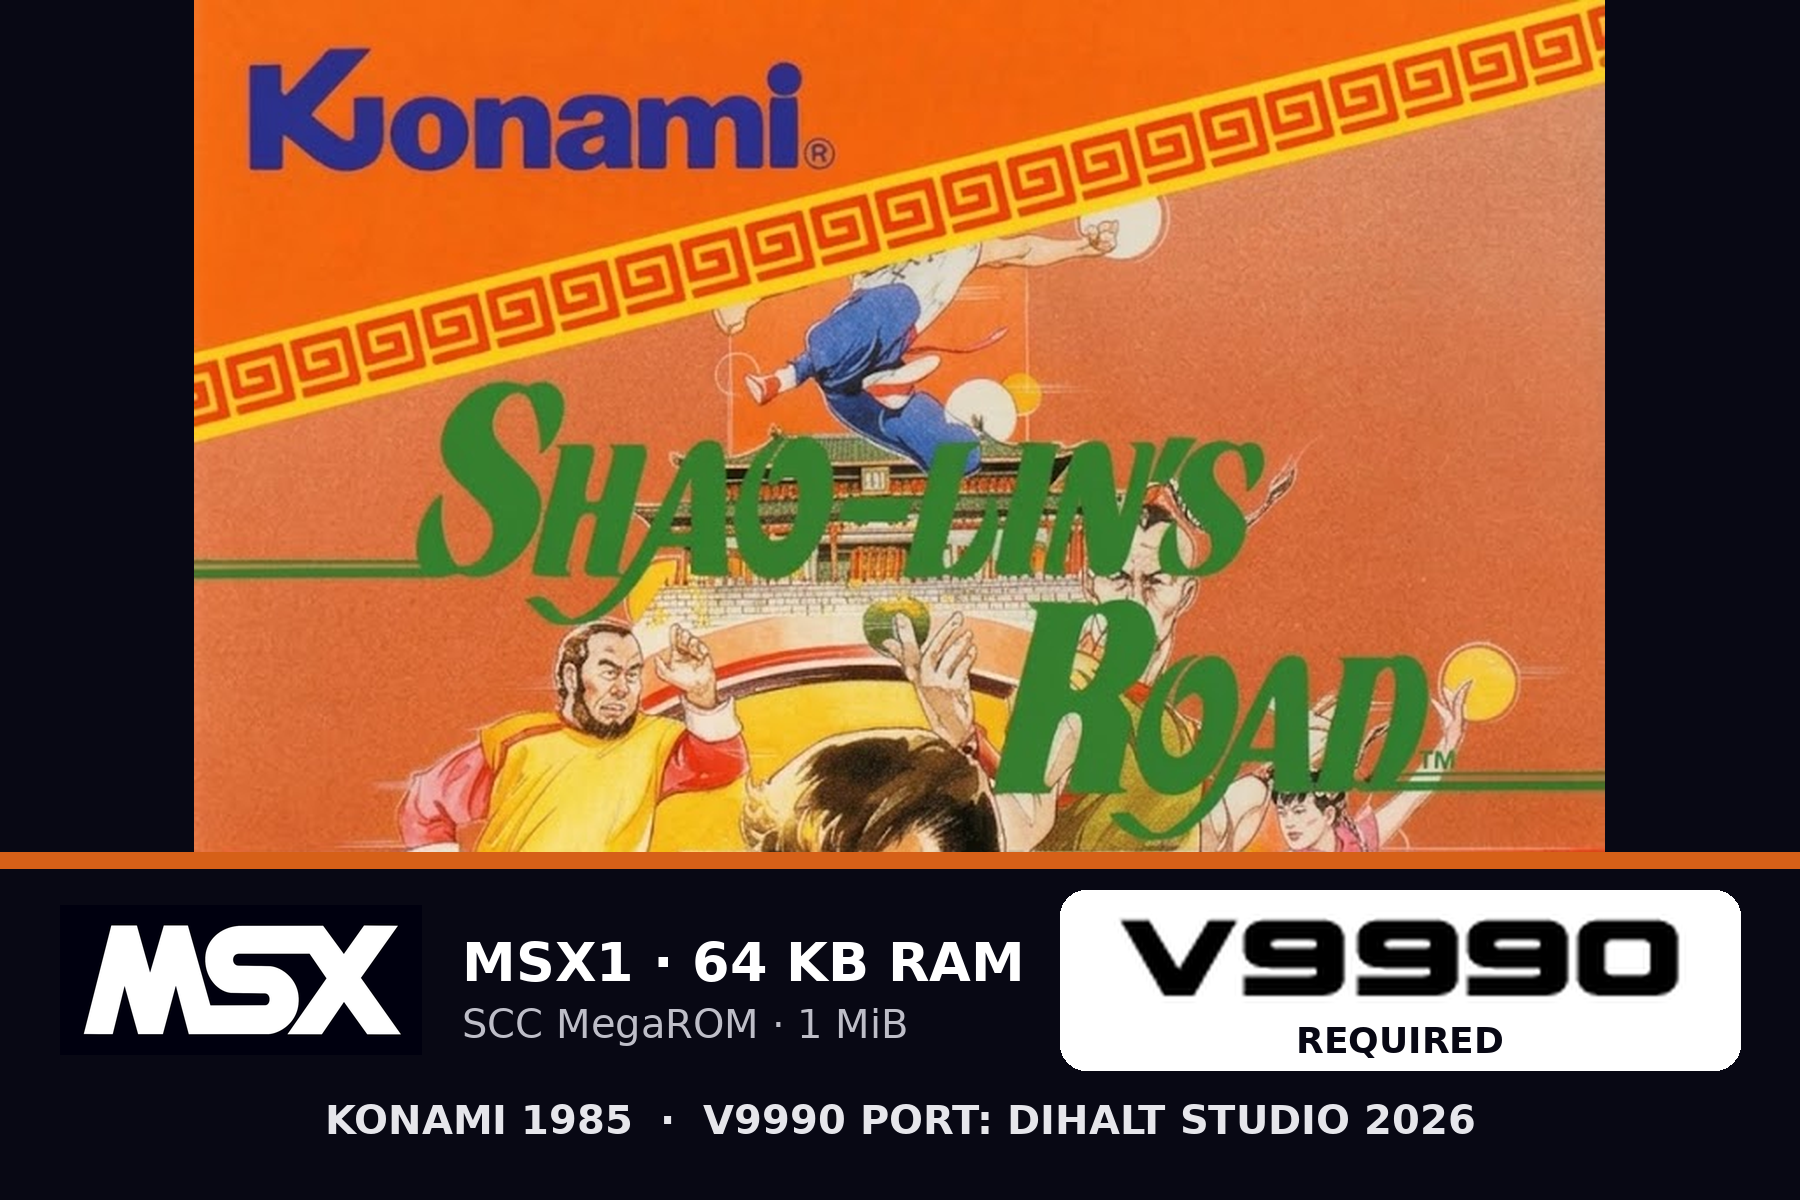
\includegraphics[width=\textwidth]{img/sticker.png}
\end{center}

\end{document}
